\documentclass[fontsize=12pt,a4paper]{scrreprt}

\usepackage[margin=1in,heightrounded]{geometry}
\usepackage{graphicx}
\usepackage{lipsum}
\usepackage[T1]{fontenc} % prevents < in text mode turning into
\usepackage{textcomp}    % ?', etc
\usepackage[osf]{mathpazo} % Palatino font
\usepackage{courier} % nicer typewriter-style fonts
\usepackage[scaled=.9]{helvet} % nice san serif fonts
\usepackage{microtype} % micro-typographical extensions
\usepackage[british]{babel} % British hyphenation patterns, etc.
\usepackage{fixltx2e}
\usepackage{enumitem}
\usepackage{tabularx}
\usepackage{booktabs}

\renewcommand*{\chapterheadstartvskip}{\vspace*{-\topskip}}

\setlength{\parskip}{1em}
\pagestyle{headings}

\author{Y0070944}
\title{IAPT Longboxes Design Document}

\begin{document}

\maketitle
\setcounter{page}{1}

%-------------------------------------------------------------------------------
\chapter{Data Model}
%-------------------------------------------------------------------------------

\section{Class Diagram}
% [x] Provide an Entity Relationship model for the conceptual design of your database. This ER model should use the UML class diagram notation as discussed in lecture and in the readings.
% [x] This logical design should minimise redundancy through normalisation and specify primary keys that maintain entity integrity and foreign keys that maintain referential integrity.

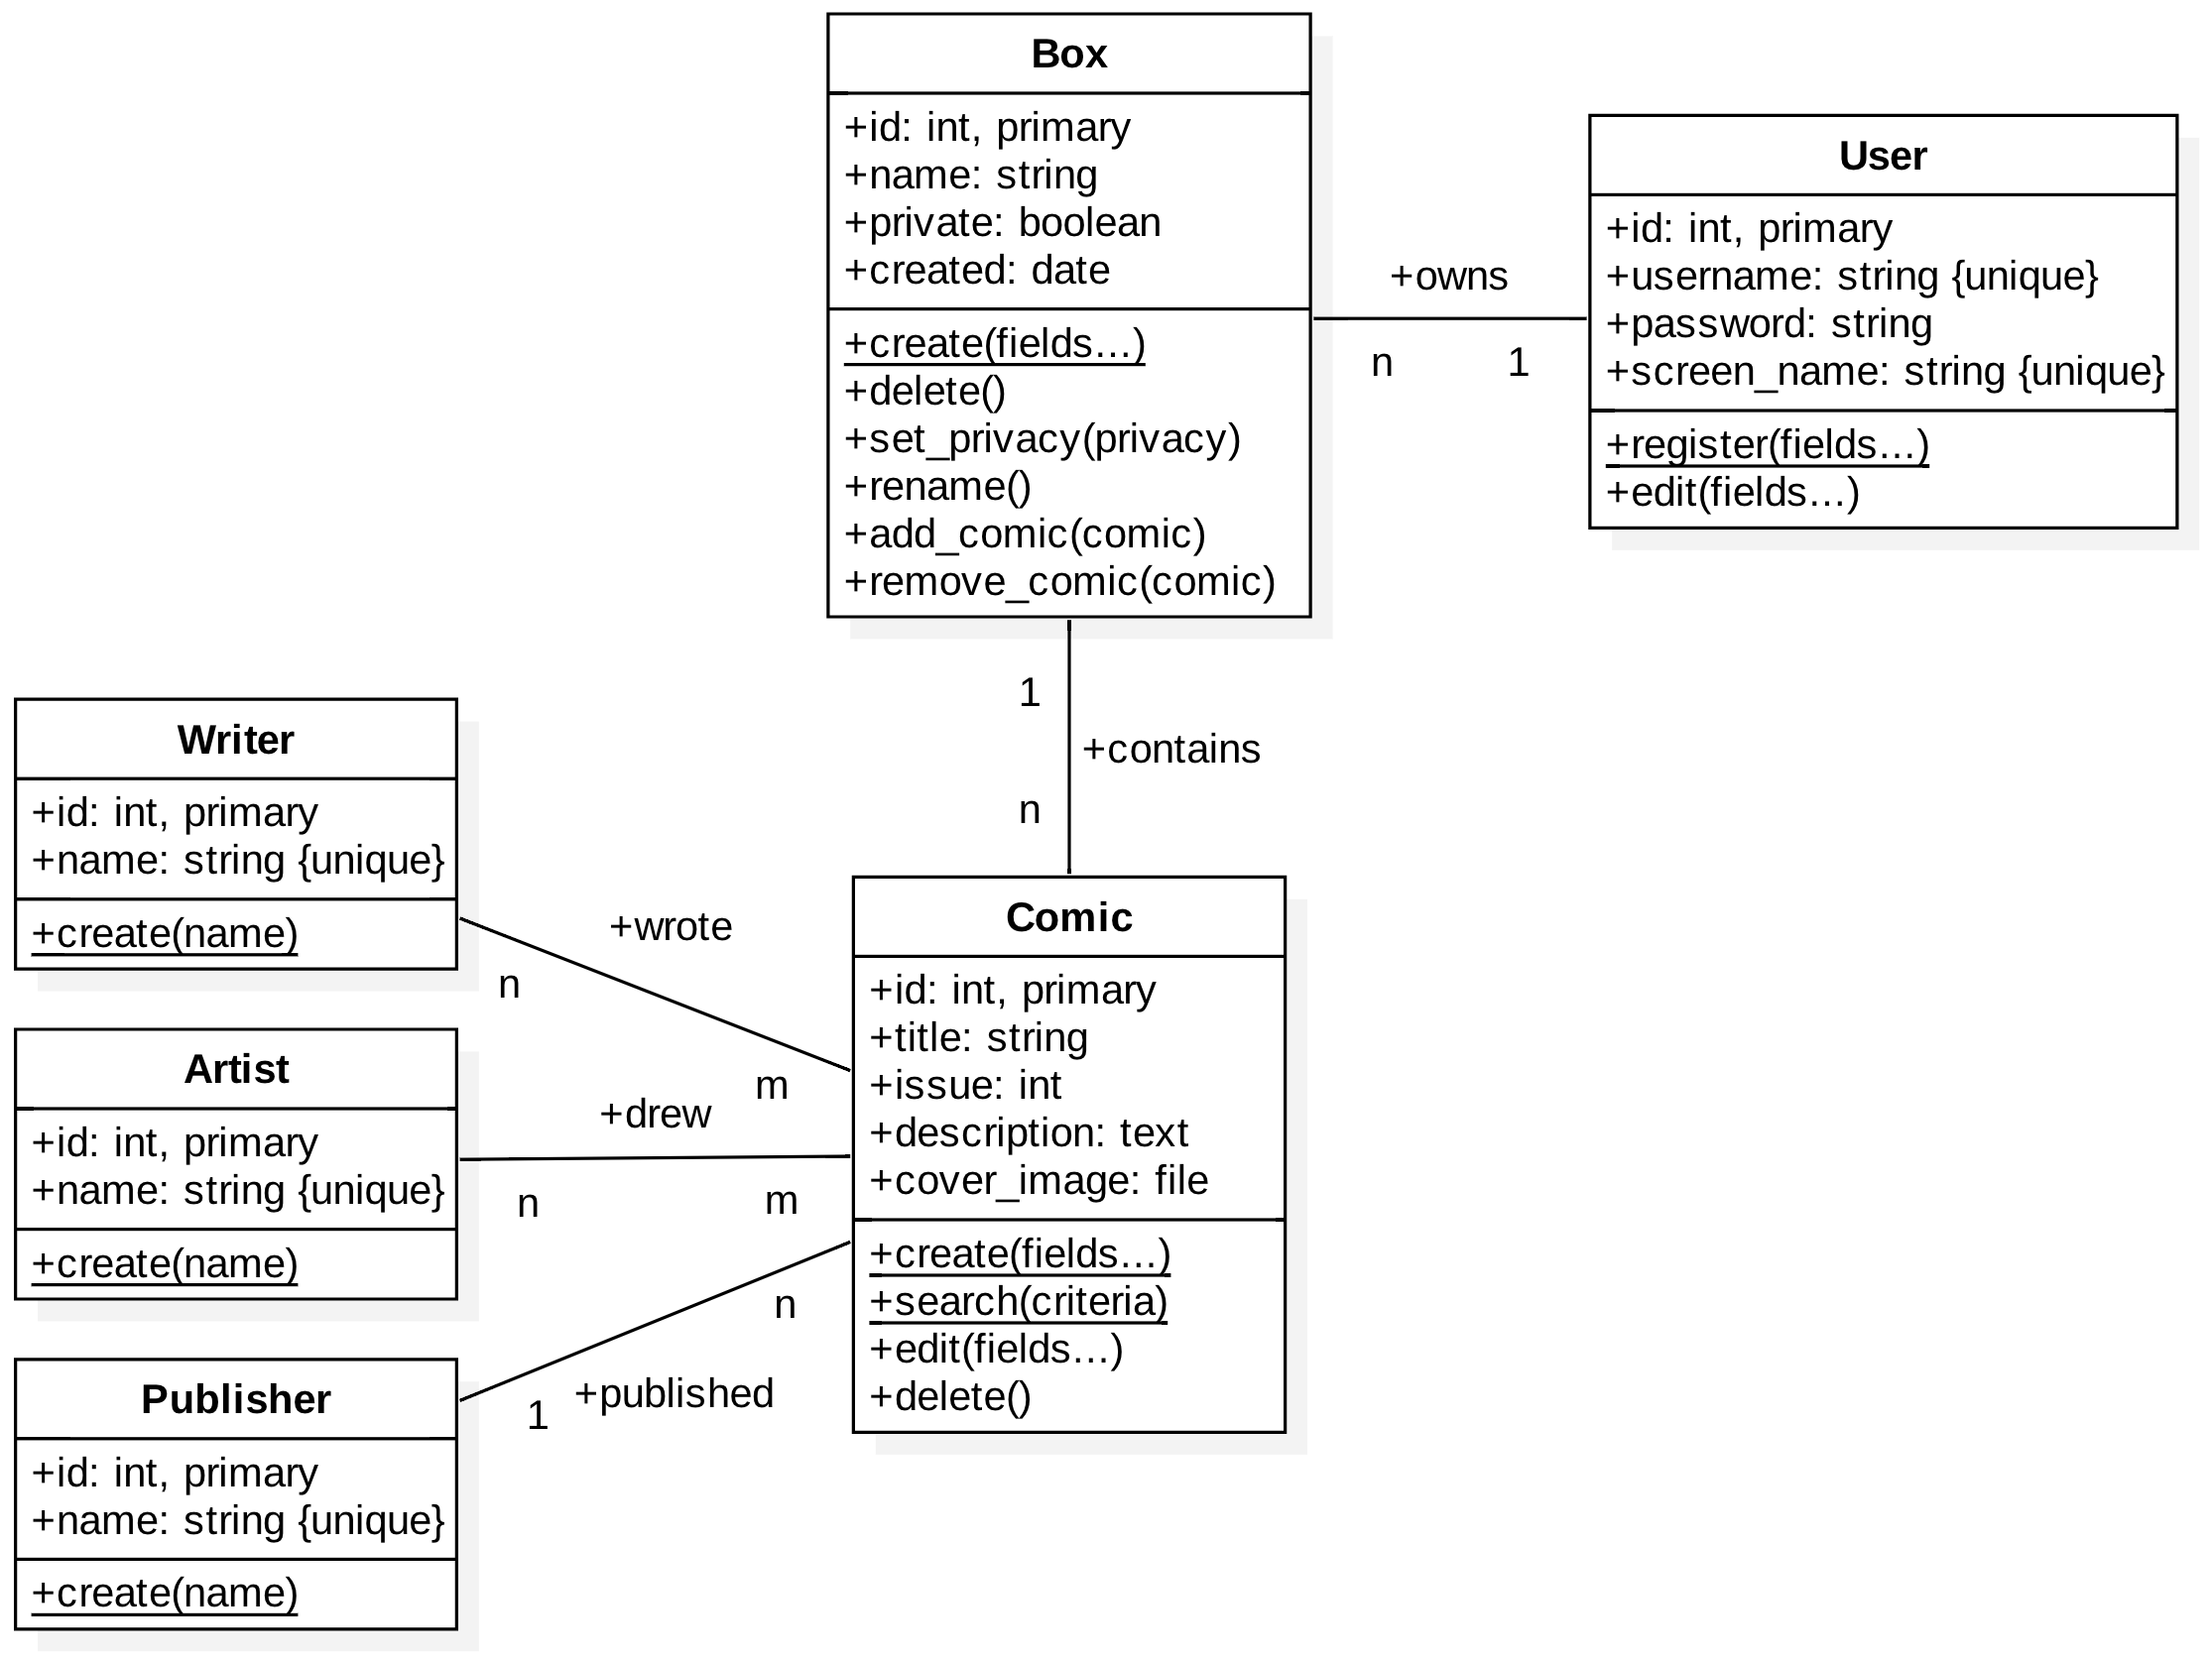
\includegraphics[width=\textwidth]{uml.png}

\subsubsection{Understanding the diagram}
\begin{itemize}[itemsep=-0.5em]
  \item Primary keys are denoted by a \textsf{primary} tag after the key name.

  \item Underlined transactions denote that they are static, i.e., do not act upon a specific instance of the entity.

  \item Labels on the edges between entities (relationships) should be read from \textsf{1 to n} or \textsf{n to m}. For example, \textsf{Publisher \emph{published} Comic}.
\end{itemize}

\subsubsection{Transaction to controller function mapping}
% [ ] Demonstrate through annotation of your conceptual model that the conceptual design correctly supports the transactions needed by your application. Provide a table that maps these transactions to controller functions in the Web2Py Python controller.

\begin{tabularx}{\linewidth}{lllX}\toprule
\textbf{Model} & \textbf{Transaction} & \textbf{Controller function} & \textbf{Comments} \\ \hline

User & register & default/user/register &  \\
User & edit & default/user/profile &  \\ \hline

Box & create & box/create &  \\
Box & delete & box/delete &  \\
Box & set\_privacy & box/set\_privacy &  \\
Box & rename & box/view & \textsf{[1]} \\
Box & add\_comic & box/add\_comic &  \\
Box & remove\_comic & box/remove\_comic &  \\ \hline

Comic & create & comic/create &  \\
Comic & search & comic/search &  \\
Comic & edit & comic/edit &  \\
Comic & delete & comic/delete &  \\ \hline

\begin{tabular}[c]{@{}l@{}}Writer\\ Artist\\ Publisher\end{tabular} & create & \begin{tabular}[c]{@{}l@{}}comic/create\\ comic/edit\end{tabular} & \textsf{[2]} \\

\bottomrule
\end{tabularx}

{
  \setlength{\parindent}{0}
  \setlength{\parskip}{0.4em}

  \textsf{[1]} This function handles box renames requested by a form in a modal dialog on the \textsf{view} page.

  \textsf{[2]} \textsf{Writer}, \textsf{Artist} and \textsf{Publisher} entities are automatically created when comics require them.
}

%-------------------------------------------------------------------------------
\chapter{User Interface Design Rationale}
%-------------------------------------------------------------------------------

\lipsum[3-6]

\end{document}
